\section{Three Saturnine Philosophers}

\begin{quotex}
Not to laugh, not to cry, not to curse, but to understand. \flright{\textsc{Baruch Spinoza}}

\end{quotex}

Saturn is the outermost or highest planet in the cosmic order, and so is nearest to the divine source of being and closest to the angelic hierarchy. Therefore, Saturn is associated with the loftiest contemplations. Saturnians are inspired students and contemplators of highest truths. To be melancholy was a sign of genius; the `gifts' of Saturn, the numbering and measuring studies attributed to the melancholic, were to be cultivated as the highest kind of learning which brought man nearest to the divine.

When I was a teenager in Stoneham, a suburb of Boston, the only bookstore in town was at the drugstore. There you could find comics, magazines, and a couple of book racks. One had self-help books from Parker Publishing, and the other rack was full of Dover reprints. There were books on mathematics, science, cryptography, logic, and philosophy; at least, those were the books that interested me.

\begin{wrapfigure}{rt}{.3\textwidth}
 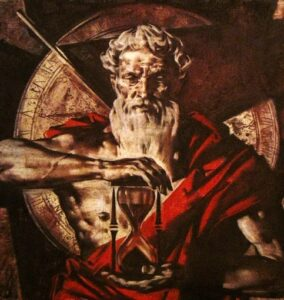
\includegraphics[scale=.5]{a20210407ThreeSaturninePhilosophers-img001.jpg}
\end{wrapfigure}

I still have many of those books. Although I liked the philosophers of logic, science, and positivism, the most influential philosophers were Spinoza, Schopenhauer, and Santayana. They were not as simple as the others, so they required some penetration to reach them. I called them the three ``esses".

What follows are the impressions left by these thinkers. I am writing from memory, so it may not be a precise summary of their philosophies in an academic. Yet the traces they left in my mind still linger. All three followed the jnani path throughout their lives, while I took some time out to follow the path of the householder. So there was a time before, then a long period of intellectual darkness, and then the light shines again.

\paragraph{Essence and Presence}

The temptation is to believe that you understand a philosopher when you can reduce him to some preconceived categories. I claim, instead, that it is necessary to wrestle with the ideas and grasp what issues are at stake. \textbf{Baruch Spinoza}'s \emph{Ethics} is an intellectual tour de force; the effort to present a system of thought like a textbook of geometry required tremendous organization and effort. Here, we can only present his main points.

\paragraph{God}
First of all, he conceives of the Whole, which he calls God. As the Whole, it cannot be dependent on anything else. Moreover, it is necessary, infinite, and self-caused. As such, he is not deviating from the classical understanding of God. Since God is infinite, there cannot be two gods.

\begin{wrapfigure}{rt}{.3\textwidth}
 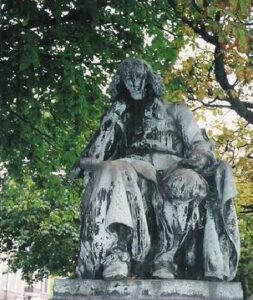
\includegraphics[scale=.5]{a20210407ThreeSaturninePhilosophers-img002.jpg}
\end{wrapfigure}

He refers to God as a substance, the only substance, in fact, and the only substance that can even be conceived. Sometimes he refers to ``God or Nature", which some interpret as pantheism. But Nature is not the physical or material world, as we understand it. Rather Nature is the opposite pole to God. Envision a vertical axis with God as essence as the north pole and Nature as the south pole. All that means is that, for God, essence and existence are the same, again a traditional understanding.

\paragraph{Attributes}
An attribute is anything that can be predicated of a substance. Since God is the only substance, He has attributes, which express His essence. Spinoza claims that there is no limit to the number of God's attributes, although he identifies just two. Following Rene Descartes, these are:

\begin{enumerate}
\item \textbf{Extension}: This attribute applies to bodies and includes its size, shape, place. 
\item \textbf{Thought}: This attribute applies to minds and includes all conscious experiences including sense data, emotions, images, thoughts, and so on. 
\end{enumerate}
In order to avoid Cartesian dualism, Spinoza claims that God or Nature can be understood under either attribute. Thus, one can understand Nature by means of matter or by thought.

Extension and Thought can best be understood as states of the Being, similar to the metaphysical distinction between the Gross and Subtle Bodies. By the Law of Correspondence, what happens at one attribute happens at the other level; the relationship, however, is not causal. As a practical matter, one may be preferable to another, depending on circumstances.

For example, consider a children's birthday party. A scientist, considering it strictly from the material point of view (Extension), will measure energy consumption and expenditure, gather auditory data, and so on. Although he can verify that the Laws of the Conservation of matter, energy, and momentum have not been violated, he will not ``know" that he was observing a birthday party. Nevertheless, there are people, even educated people, who remain convinced that the world can be understood as merely the movement of atoms. String theory will never be able to predict nor to explain such a party.

The mothers and children, on the other hand, will experience various emotions and sensory stimuli. The mothers feel pride at their children and the children experience joy. They will not have violated any laws of physics at the party.

There is yet a higher way to understand things and events, but that will come later.

\paragraph{Modes and the Unity of Being}
Since God is the only substance, individual things are merely modes, which can appear as bodies or as minds. A mode has less reality than God, who alone is full real.

Spinoza here is remarkably close to Traditional metaphysics such as that described by \textbf{Shankara}. He is actually closer here to \textbf{Ibn Arabi}'s understanding of the Unity of Being. Since God is Being itself, individuals do not possess full reality; only God is fully real. Ibn Arabi was a Sufi and this is Sufi metaphysics (or, at least, that of one of its schools).

There is no place here to resolve the relationship between Being and individual beings.

\paragraph{The Degrees of Knowledge}
Like all Tradition, Spinoza identified three degrees of knowledge:

\begin{enumerate}
\item \textbf{Opinion}: This is our knowledge of the objects of sense and theories derived from them. This includes scientific theories. 
\item \textbf{Reason}: This includes knowledge derived from thinking and logic. 
\item \textbf{Intuition}: This is a direct, unmediated knowledge. Since the Whole has no parts, it cannot be fully known through reason. Instead, one must understand the Whole, or God, directly without the intervention of thought. 
\end{enumerate}
\paragraph{Sub specie aeternitatis}
To circle back to the birthday party, Spinoza claims to know things ``\emph{sub specie aeternitatis}", that is, from the perspective of eternity. This is more than a philosophical theory, since Spinoza is claiming to understand things from God's perspective. In effect, he claims to be a prophet of God.

\paragraph{Conatus}
A mode strives to persevere in being. This striving, or inner drive, is called Conatus.

Hence, physical objects do not ``follow rules" or laws, rather they act out of inner necessity. Ideally, this is also true for Minds. The will is not free insofar as it is determined by some motive. In most cases, a person is unaware of the true causes of his actions. In other words, he does not know himself.

In particular, the human being is driven by emotions. These can be active or passive. This is described in Wikipedia:

\begin{quotex}
the most important distinction is that between ``active" feelings and ``passive" feelings (or ``passions"). Man, according to Spinoza, is active or free in so far as any experience is the outcome solely of his own nature; he is passive, or a bondsman, in so far as any experience is due to other causes besides his own nature. The active feelings are all of them forms of self-realisation, of heightened activity, of strength of mind, and are therefore always pleasurable. It is the passive feelings (or ``passions") which are responsible for all the ills of life, for they are induced largely by things outside us and frequently cause that lowered vitality which means pain.

\end{quotex}
When a Man is free, his actions arise from his own essence; he has transcended his passive feelings. For him, morality is no longer a matter of following rules. Rather comes from within. Of course, this requires a process of the purification of the mind, will, and emotions.

\paragraph{The Love of God}
For Spinoza, the intellectual love of God combines the highest form of knowledge with the greatest emotion. In effect, this is God contemplating himself in the being. Our love for God, therefore, is God's love for humanity.

Salvation therefore consists in a constant and eternal love of God. This is the most elevated and desirable state, and is the goal of the \emph{Ethics}.

To be continued.

\flrightit{Posted on 2021-04-07 by Cologero }
